\documentclass[12pt]{scrartcl}%{article} % Beginn der LaTeX-Datei
%Titel etc

\title{
\begin{flushright}
 \includegraphics[scale=0.5]{HAW_Marke_RGB_300dpi.jpg}
\end{flushright}

\vspace{2cm}

IT-Systeme\\
Dokumentation
 
\vspace{1cm}

\LARGE Interaktive Videoinstallation mit\\
granularem Synthesizer
}

%\author{}
\date{23. Februar 2024}

% Kopf- und Fußzeilen

\usepackage[headsepline,%footsepline
]{scrlayer-scrpage}
\pagestyle{scrheadings}
\clearpairofpagestyles


\ihead{23.02.2024}
\chead{IT Systeme}
\ohead{Dokumentation: visueller Synthesizer}
\ifoot{}
\cfoot{}
\ofoot{\pagemark}

%% twocolumn

\usepackage{amsmath,amssymb}  % erleichtert Mathe 
\usepackage{enumerate}% schicke Nummerierung

\usepackage{graphicx} % für Grafik-Einbindung
%\usepackage{hyperref}

\usepackage[german]{babel}
\usepackage[T1]{fontenc}
\usepackage{lmodern}
\usepackage{textcomp}
 % Einstellungen, wenn man deutsch schreiben will, z.B. Trennregeln
\usepackage[utf8]{inputenc}  % für Unix-Systeme
  % ermöglicht die direkte Eingabe von Umlauten und ß
  % evt. obige Zeile ersetzen durch
  % \usepackage[ansinew]{inputenc}  % für Windows
  % \usepackage[applemac]{inputenc} % für den Mac


%%%%%%%%%%%%%%%%%%%%%%%%%%%%%%%%%%%%%%%%%%%%%%%%%%%%%%%%%%%%%%%%%%
%
%  ntheorem
%
\usepackage[thmmarks,amsmath,hyperref,noconfig]{ntheorem} 
  % erlaubt es, Sätze, Definitionen etc. einfach durchzunummerieren.
\newtheorem{satz}{Satz}[section] % Nummerierung nach Abschnitten
\newtheorem{hilfssatz}[satz]{Hilfssatz}
\newtheorem{kor}[satz]{Korollar}

\theorembodyfont{\upshape}
\newtheorem{beispiel}[satz]{Beispiel}
\newtheorem{bemerkung}[satz]{Bemerkung}
\newtheorem{definition}[satz]{Definition} %[section]

\theoremstyle{nonumberplain}
\theoremheaderfont{\itshape}
\theorembodyfont{\normalfont}
\theoremseparator{.}
\theoremsymbol{\ensuremath{_\blacksquare}}
\newtheorem{beweis}{Beweis}
\qedsymbol{\ensuremath{_\blacksquare}}
%\theoremclass{LaTeX}
%
% Ende ntheorem
%
%%%%%%%%%%%%%%%%%%%%%%%%%%%%%%%%%%%%%%%%%%%%%%%%%%%%%%%%%%%%%%%%%%


%\pagestyle{empty}
%
% Ändern der bedruckten Fläche der Seite
% \addtolength{\textwidth}{3cm}  % Befehl mit zwei Argumenten
% \addtolength{\textheight}{3cm}
% \hoffset-2cm % verschiebt das Textfenster nach links
% \voffset-5mm % verschiebt das Textfenster nach oben
%
%\parindent=0pt %% keine Einzug zu Beginn von Abs\"atzen
%\parskip=2mm   %% erzeugt einen zusätzliche Zeilenabstand zwischen
                %% Absätzen. Nötig bei \parindent=0pt


%%%%%%%%%%%%%%%%%%%%%%%%%%%%%%%%%%%%%%%%%%%%%%%%%%%%%%%%%%%%%%%%%%
% ermöglicht, farbigen Text zu drucken.
\usepackage{color}
% Und nun werden die Farben definiert - daran können Sie nach Belieben selber rumspielen.
\definecolor{white}{rgb}{1,1,1}
\definecolor{darkred}{rgb}{0.3,0,0}
\definecolor{darkgreen}{rgb}{0,0.3,0}
\definecolor{darkblue}{rgb}{0,0,0.3}
\definecolor{pink}{rgb}{0.78,0.09,0.51}
\definecolor{purple}{rgb}{0.28,0.24,0.55}
\definecolor{orange}{rgb}{1,0.6,0.0}
\definecolor{grey}{rgb}{0.4,0.4,0.4}
\definecolor{aquamarine}{rgb}{0.4,0.8,0.65}

\usepackage[table]{xcolor}% http://ctan.org/pkg/xcolor
\usepackage{lipsum}
\usepackage{wrapfig}
\usepackage{hyperref}



\DeclareMathOperator{\GL}{GL} % einige Macro, siehe am Ende Abschn. 2
\newcommand{\N}{\mathbb{N}}
\newcommand{\Z}{\mathbb{Z}}
\newcommand{\Q}{\mathbb{Q}}
\newcommand{\R}{\mathbb{R}}
\newcommand{\C}{\mathbb{C}}
\newcommand{\cP}{{\mathcal P}}


\begin{document}

\begin{titlepage}


\maketitle % erzeugt den Kopf


\vfill 

\begin{flushleft}
\begin{tabular}{rlll}
%\cline{1-3}
\textbf{Gruppe:} & Ariane Bachmann & 2552756 & \hspace{5cm} \\
 & Benjamin Ghodsi-Moghaddam & 2582359 & \hspace{5cm} \\
 & Bruno Bühler & 2625322 & \hspace{5cm} \\
  & Dennis Jonca & 2175314 & \hspace{5cm} \\
   & Evan Tanggo Peter Simamora & 2332397 & \hspace{5cm} \\
    & Fabian Brunner &  2600389 & \hspace{5cm} \\
& Rafael Weber & 2623881 & \hspace{5cm} \\\\
%\cline{1-3}
\textbf{Studiengang:} & Meidentechnik B.Sc. WS 23/24 & \hspace{5cm} \\\\
%\cline{1-3}
\textbf{eingereicht bei:} & Malte Sanders & \hspace{5cm} \\ 
%\cline{1-3}
\end{tabular}
\end{flushleft}

\end{titlepage}

\tableofcontents

\newpage

\section{Einleitung}

Das Projekt „VisuSynth“ des Kurses IT-Systeme ermöglicht es, eine Interaktion zwischen
Klängen, Bildern und der eigenen Kreativität zu erschaffen. Dabei können Töne live aufgenommen, bearbeitet und in visuelle Bewegungen umgewandelt werden.
\\\\
Ziel war es, das Projekt durch eine verständliche Bedienung auch für Unerfahrene im Bereich Audiosynthese verständlich und bedienbar zu machen. Außerdem sollten die Nutzer ermutigt werden, eigene Ideen zu entwickeln.

\section{Grundlagen}

Der Bereich Audio-Synthese sowie die Schnittstelle MIDI waren nicht dem ganzen Projektteam bekannt. Deshalb war es wichtig, Informationen über diese Bereiche zu sammeln, damit auf einem ähnlichen Wissensstand gearbeitet werden konnte.

\subsection{Granular-Synthese}

Die Granular-Synthese ist eine Synthese-Form wie z.B. auch die Subtraktive Synthese, FM-Synthese (Frequenzmodulation) oder auch die Wellenform Synthese, die zur musikalischen Klangerzeugung dienen. Einige diese Formen haben sich dabei stark oder weniger stark durchgesetzt. Es dabei wichtig zu unterscheiden, ob analoge oder digitale Synthese verwendet wird.
\\\\
In den 1960er Jahren wurden die ersten analogen Synthesizer vorgestellt. Am einflussreichsten war dabei der Ingenieur Robert Moog, der bis heute als Pionier in der Welt der Synthesizer und elektronischen Musik gilt. Moog Synthesizer sind bis heute beliebt. Die Klangerzeugung basiert dabei auf die Verschaltung von elektronischen Bauteilen.
Mit einer Weiterentwicklung von Computern und der Erfindung erster serienmäßig produzierbaren Mikroprozessoren, kam es auch zu Erfindung erster Synthesizer, die auf digitaler Synthese beruhten. Einen Meilenstein legte dabei der Yamaha DX7. Ein Algorithmus auf einem Mikroprozessor stellt hier per FM-Synthese den Klang her.
\\\\
Die Granular-Synthese beruht darauf, ein Sample(„Audioschnipsel“) in kleine „Grains“ zu unterteilen, die zwischen 1ms – 50ms lang sind. Diese können dann in verschiedenen Tonhöhen, Geschwindigkeiten oder an verschiedenen Positionen abgespielt werden. Dies sorgt häufig für atmosphärische oder auch experimentelle Klänge. Es benötigt zur granularen Synthese ein vorher aufgenommenes oder gespeichertes Sample.

\subsection{Umsetzung}

Um diese Synthese-Form zu benutzen war es auch wichtig zu unterscheiden, wie man digitale Synthese umsetzen kann. Eine Möglichkeit wäre gewesen, einen DSP zu verwenden, auf dem der Algorithmus dann läuft, ähnlich wie beim Yamaha DX7. Dies setzte tiefgehende Programmierkenntnisse, sowie die Fähigkeit einen solchen Algorithmus erstellen zu können, Voraus. 
Eine andere Möglichkeit war es, eine schon vorhandene Umgebung/ Softwareanwendung zu verwenden, die die Synthese dann auf der CPU des PC’s/Laptops durchführt. Zusätzlich haben viele dieser Umgebungen auch vorgefertigte Module und Anleitungen, um eigene Synthesizer zu bauen.
\\\\
Mögliche Tools sind dabei Max for Live (Ableton, Cycling’74), Reaktor (Native Instruments) oder SunVox (Alexander Zolotov).

\subsection{MIDI}

MIDI („Musical Instrument Digital Interface“) ist eine Schnittstelle, die zur Übertragung von musikalischen Informationen dient. Dabei gibt es verschiedene Datentypen, die über MIDI übertragen werden. Für das Projekt waren vor allem die Werte „Control Change“ sowie „Note On“ und „Note Off“ wichtig. 

\newpage

\section{Konzeption}

Die Besucher betreten einen abgedunkelten Raum, in dessen Mitte sich, beleuchtet von zwei Scheinwerfern, ein Stehtisch befindet, der die notwendigen Bedienelemente beherbergt. Über einen Projektor werden zunächst Standby-Versionen der Visuals an eine Leinwand im vorderen Teil des Raumes projiziert, die später im Einklang mit dem Audio dynamisch verändert werden.
\\\\
Zur Verfügung stehen den Nutzern verschiedene Bedienelemente, darunter ein Mikrofon zur Aufnahme einer Audiospur als Basis für den Granular-Synthesizer, sowie eine kleine Auswahl an Instrumenten und klangbildenden Objekten wie z.B. eine Steel Drum, ein Mini-Cajon, eine Ukulele, ein Kalimba usw. Ein MIDI-Keyboard ermöglicht die Kontrolle der Tonhöhe des Synthesizers. Zusätzlich gibt es einen Mikrocontroller mit sechs Potentiometern zur Steuerung der Synthesizer-Parameter (Frequenz, Spray, Mode, Reverb, Delay, Bitcrush), einem Schieberegler zur Positionierung innerhalb der Audiospur und einem Button zur Steuerung des Visualwechsels.
\\\\

\begin{center}
 \includegraphics[scale=0.11]{Rauminstallation}
 \captionof{figure}{Rauminstallation}
\end{center}

\newpage

\noindent Der Ablauf beginnt mit der Aufnahme einer Audiodatei über das Mikrofon, indem der Nutzer über den Laptop den Record-Button in der Software SunVox drückt. Nachdem die Aufnahme gestoppt wurde, zeigt der Laptop die Waveform der Audiodatei an. Er ist ab diesem Punkt nur noch Rechenzentrum der Installation, während die Bedienung ausschließlich über das MIDI-Keyboard und den Mikrocontroller erfolgt.
\\\\
Die MIDI-Daten des Mikrocontrollers und des Keyboards werden an den Laptop gesendet, auf dem die Audiosynthese der zuvor aufgenommenen Audiodatei stattfindet. Das resultierende Audiosignal wird über Lautsprecher in den Raum gegeben und gleichzeitig intern an TouchDesigner weitergeleitet. Dort wird das Audiosignal in Echtzeit hinsichtlich seines Frequenzspektrums und seiner Dynamik analysiert und in sechs verschiedene visuelle Darstellungen umgewandelt, die live gerendert und auf eine etwa 2x2m große Leinwand am vorderen Ende des Raumes projiziert werden.
\\\\
Die Visuals wechseln nun automatisch alle zwei Minuten, können aber auch direkt vom Nutzer über einen Button auf dem Mikrocontroller gesteuert werden.
\\\\

\begin{center}
 \includegraphics[scale=0.5]{Blockschaltbild}
 \captionof{figure}{Blockschaltbild des kompletten Systems}
\end{center}

\newpage

\section{Projektdurchführung}

Zum Sammeln und Strukturieren von Ideen wurde das Tool „Miro“ verwendet. Dort konnten erste Ideen skizziert und eine grobe Aufteilung der Aufgabengebiete dargestellt werden. In der ersten Phase des Projektes war es dabei wichtig zu sondieren, welche Möglichkeiten es gibt und welche Werkzeuge dafür benötigt werden. Ein Miroboard war dabei hilfreich, um im Team zu kooperieren und alle Ideen übersichtlich zu halten.
\\\\
Im Anschluss wurde ergänzend ein Git-Repository angelegt, um alle Materialien, Dateien und Texte abzulegen und für alle Mitglieder des Teams zugänglich zu machen.
\\\\
Eine Gruppeneinteilung half frühzeitig, um eine klare Arbeitsaufteilung untereinander sicher zu stellen. Dabei wurde sich auf folgende Teams festgelegt: 
\begin{itemize}
  \item \textbf{Software}: Recherche nach Software zur Granular-Synthese sowie Erstellung eines Granular-Synthesizers.
  \item \textbf{Hardware}: Planung und Umsetzung eines Controllers mit geeignetem Layout, der Wert von Drehreglern und Fadern per MIDI an einen Computer sendet.
  \item \textbf{Visuals / TouchDesigner}: Erstellung von verschiedenen TouchDesigner-Projekten, die Audio verarbeiten und dazu geeignet reagieren.
\end{itemize}

\subsection{Zeitplanung}

Für das Management und die Zeiteinteilung wurden einige Ideen aus Scrum genutzt. So traf das Team sich beispielsweise einmal die Woche zu einem Meeting, um den aktuellen Fortschritt, bestehende Herausforderungen sowie potenzielle Lösungsansätze zu erfassen.
\begin{wrapfigure}{r}{0.7\textwidth}
  \centering
  \includegraphics[width=0.6\textwidth]{road1}
  \caption{Auszug der Roadmap}
\end{wrapfigure}

\noindent Des Weiteren wurde eine Roadmap erstellt, die den zeitlichen Rahmen für jedes Team visualisierte. Dabei war es entscheidend, ausreichend Pufferzeiten einzuplanen, da in der Praxis Verzögerungen unvermeidlich sind oder bestimmte Projektabschnitte nicht wie geplant verlaufen könnten.
\\\\

\newpage

\subsection{Software}

Es wurde schnell klar, dass eine Synthese innerhalb des Mikrocontrollers sehr komplex werden könnte. Deshalb wurde festgelegt, die Audio-Synthese auf der CPU des PCs über eine Software zu gestalten. Nachdem verschiedene Umgebungen getestet wurden, hat man sich auf die Software SunVox geeinigt.\\
SunVox bietet umfassende Möglichkeiten, um individuelle Synthesizer zu bauen. Dabei bleibt es verständlich und im Vergleich zu anderen Programmen leicht zu erlernen. Zudem ist SunVox kostenlos nutzbar. Dies war auch ein wichtiger Faktor, damit alle Personen uneingeschränkt mit dem Programm arbeiten konnten.

\subsubsection{SunVox Implementierung}

Nach der Entscheidung, SunVox als Synthesizer Software zu nutzen, galt es zuerst, ein Projekt zu bauen, das die Hauptaspekte der granularen Synthese erfüllt und steuern lässt. Also dass ein Sample zu einem gewählten Punkt in einer bestimmten Frequenz abgespielt werden kann. Das Sample sollte dabei entweder selbst aufgenommen oder ausgewählt werden. Dies ließ sich prinzipiell einfach mit den in SunVox eingebauten Modulen umsetzen.

\begin{wrapfigure}{r}{0.7\textwidth}
  \centering
  \includegraphics[width=0.65\textwidth]{sunvox_1}
  \caption{Aufbau des Granulator Moduls in SunVox}
\end{wrapfigure}
\noindent Es gibt in SunVox das sogenannte MultiSynth Modul, welches allgemein genutzt werden kann, um ein Audiosample abzuspielen und dabei bestimmte Eigenschaften verschiedener Module zu transportieren und auf das jeweilige Sample zu übertragen.\\
Es kann außerdem direkt die angespielte Phase eingestellt werden, weshalb sich darüber endlich auch die Position des Samples bestimmt, die hardwareseitig vom Slider kontrolliert werden sollte. Dass das Sample dann aber nicht nur einmal abgespielt wird, sondern in sich wiederholenden Grains, wird durch einen Low Frequency Oscillator sichergestellt, der auch als Modul in SunVox vorhanden ist. Sobald der MultiSynth gespielt wird, wird auch der LFO angesteuert und triggered in einer einstellbaren Frequenz das Sample immer wieder neu an. Wie lang das Sample abgespielt wird, bestimmt sich im Endeffekt aus der gewählten Frequenz des LFO, um aber darüber hinaus noch mehr vom Sample in einen eingestellten Sound hineinzubekommen, lässt sich die gewählte Position, die Phase des MultiSynth, auch mehr oder weniger randomisieren, was zu einer Art Position Spray führt, was noch mehr Abwechslung in die Soundgestaltung bringen sollte.
\\\\
Ein großer Pluspunkt für SunVox ist die einfache Anbindung von MIDI-Geräten. Ein jeweiliger Controller muss nur am Rechner angeschlossen sein und man kann Parameter für Parameter auf die Bedienelemente legen wie man will. Dabei hätte man sogar experimentell mehrere Parameter auf ein Potentiometer mappen können. Für das MIDI-Keyboard, das zum Spielen verwendet werden sollte, musste nur festgelegt werden, welches Modul die Keyboard-MIDI-Befehle annehmen soll. Das war entsprechend unser selbst gebautes Granulator Modul.\\
\begin{wrapfigure}{r}{0.7\textwidth}
  \centering
  \includegraphics[width=0.65\textwidth]{sunvox_4}
  \caption{Anzeige der Waveform des Samples in SunVox}
\end{wrapfigure}

\noindent Das Sampler Modul von SunVox stellt exakt die gewünschten Funktionen zum Aufnehmen und Reinladen von Samples bereit. Problem hier war aber, dass diese Funktionen nur per Mausklick im Interface auswählbar sind, was die Vorstellung einer vollends über Bedienelemente am Mikrocontroller gesteuerten Installation störte. Eventuell wäre es möglich gewesen, wenn man, statt direkt mit der SunVox Software zu arbeiten, die ebenso vorhandene Library genutzt hätte, die sich über Code steuern lässt.
\\\\
Die Entscheidung fiel dann aber schnell darauf, mit dem Programm weiterzuarbeiten und die Installation anzupassen und flexibler zu gestalten. Dies war einerseits übersichtlicher und gerade im Zusammenspiel mit der Peripherie um einiges schneller und flexibler in der Konfiguration und Fehleranalyse. Es hätte zudem deutlich mehr Zeit benötigt, sich in den Code der Software hineinzuarbeiten, um am Ende eventuell festzustellen, dass die Installation trotzdem nicht wie geplant umgesetzt werden kann.
\\\\
SunVox bietet mit dem Sampler die Möglichkeit, die Waveform des Samples anzeigen zu lassen, inklusive Cursor, der anzeigt, wo das Sample aktuell abgespielt wird. Eine solche Visualisierung war von Anfang an für die Installation vorgesehen, nur war nicht eindeutig, wie sie eingebunden werden kann. So fiel dann die Entscheidung, einen extra Bildschirm respektive den Laptop, über den die Software am Ende lief, aufzustellen, um die Steuerung und damit die Funktionalität der Installation sicher zu stellen und gleichzeitig noch die Waveform anzeigen zu können.\\
\begin{wrapfigure}{r}{0.5\textwidth}
  \centering
  \includegraphics[width=0.45\textwidth]{sunvox_3}
  \caption{Parameter des\\Granulator Moduls}
\end{wrapfigure}

\noindent Somit stand schnell ein Projekt, dass grundlegend als Granular Synthesizer funktioniert. Von da an war die Hauptaufgabe, auszuloten, welche ansteuerbaren Parameter sich in SunVox am besten für die Bedienung an unserer Hardware eignen. Viele Optionen standen zur Auswahl, die teilweise stark den Sound beeinflussten, wie zum Beispiel die Randomisierung der Tonhöhe. Um es nicht zu kompliziert zu halten, da es ohnehin mit einem gewissen Anspruch verbunden ist, den Synthesizer zu spielen, wurden am Ende aber nur die wichtigsten Parameter Position, Loop Frequency, Position Spray sowie die, die den Sound nochmal abrunden, Reverb, Delay und Distortion gemappt (letztere waren ebenfalls direkt als Modul in SunVox vorhanden)
\\\\
\begin{figure}[h]
\includegraphics[width=\textwidth]{sunvox_2}
  \caption{Aufbau des Synthesizers in Sunvox}
\end{figure}
\newpage
\noindent Um zusätzlich das Problem zu beheben, dass es zu Artefakten in der Audio kommt, wenn das Sample durch die gewählte Position bei hoher Amplitude abgehakt wird, wurde noch versucht, mit einem ADSR Attack und Release für die Grains einstellbar zu machen, allerdings hat dieser nicht wie erwartet für die einzelnen Grains gegriffen, sondern nur für einen gespielten Input, der natürlich viele Grains hintereinander triggered.\\
\begin{wrapfigure}{r}{0.7\textwidth}
  \centering
  \includegraphics[width=0.65\textwidth]{sunvox_5}
  \caption{Manuelle Einstellung der Hüllkurve eines\\Samples}
\end{wrapfigure}

\noindent Als Alternative lässt sich die Hüllkurve des Samples zwar direkt im Sampler selbst einstellen, dies muss aber jedes Mal aufs Neue manuell gemacht werden, sobald ein neues Sample geladen wird. Das wurde dann aber entsprechend in Kauf genommen und es blieb bei den genannten Parametern, die die Hardware steuern sollte.\\

\subsection{Hardware}

Im Bereich der Hardware-Umsetzung wurden die Rahmenbedingungen durch die Ansteuerung des Synthesizers festgelegt. Dabei waren Drehregler, Schieberegler und Buttons vorgesehen, um die Effekte und Mechanismen des Gerätes bedienbar zu machen.

\subsubsection{Ausgangssituation und Anforderungen}

Während der ersten Wochen der Entwicklungsphase auf dem Miroboard wurde entschieden, dass der Synthesizer MIDI-Daten ausgeben sollte. Dies sei besonders sinnvoll, da sowohl SunVox als auch Touch Designer dieses Format effektiv nutzen können.
\\\\
Ursprünglich fiel die Wahl des Mikrocontrollers auf den ESP32 aufgrund seiner kostengünstigen Verfügbarkeit und der Annahme, dass er für sämtliche Funktionen ausreichen würde. Allerdings stellte sich später heraus, dass der ESP über eine USB-to-UART-Schnittstelle mit dem Computer verbunden wurde. Das bedeutete, dass er keine native, vollwertige USB-Schnittstelle bot, die für die Verarbeitung von MIDI-Daten erforderlich war. Daher wurde auf den Teensy 4.1 ausgewichen.
\newpage
Bereitgestellt wurden dann:
\begin{itemize}
  \item mehrere Drehpotentiometer
  \item ein Schiebepotentiometer
  \item ein einfacher Button
  \item eine 18x24 Lochrasterplatine
  \item Buchsenleisten und Steckverbinder (Jumper)
  \item diverse Kabel
\end{itemize}

\subsubsection{Proof of Concept (mit Code)}

Zunächst entstand ein einfacher C++-Programmcode in der Browseranwendung Wokwi, der dort durch die Simulation mittels einiger Regler getestet wurde.\\

\begin{wrapfigure}{r}{0.7\textwidth}
  \centering
  \includegraphics[width=0.65\textwidth]{wokwi}
  \caption{Simulation in Wokwi}
\end{wrapfigure}

\noindent Anschließend wurde mittels eines Breadboards eine initielle Schaltung mit einem Drehregler und einem Schieberegler aufgebaut und der Programmcode wurde in die Arduino IDE übertragen.
\noindent In diesem Schritt erfolgte die Erweiterung des Codes um die MIDI-Funktionalität. Hierbei wurden die Bibliotheken USB-MIDI und MIDI Library von lathoub sowie die Bibliothek MIDIUSB von Gary Grewal importiert. Diese sind direkt in die IDE integriert und erforderten keine externe Einbindung.
\\\\
Der Code wurde daraufhin getestet und mittels serieller Ausgabe überprüft.
\\\\
Die Potentiometer wurden als analoge Signale ausgelesen und ihre Werte wurden als MIDI-Daten übermittelt. Der Mikrocontroller fungierte somit als externer MIDI-Controller.

\newpage
\noindent Hier ist ein Codeausschnitt, der für ein einzelnes Potentiometer funktioniert. Er kann nach Bedarf erweitert werden.
\begin{figure}[h]
\centering
  \includegraphics[scale=0.5]{code_1}
  \caption{Kompletter Code für einen analogen Eingang}
\end{figure}\\
Für den Synthesizer wurden final insgesamt acht Inputs genutzt.
\begin{figure}[h]
\centering
  \includegraphics[scale=0.5]{code_2}
  \caption{Alle initiierten Eingänge}
\end{figure}
\newpage

\subsubsection{Aufbau}

Die grundlegende Struktur des Aufbaus war sehr einfach. Es gab jeweils acht analoge Eingänge, die alle mit 3,3V und Masse verbunden waren (Abb. 12, obere zwei Strecken). Jeder der acht Widerstände hatte einen eigenen Signaleingangspin am Mikrocontroller (Abb. 12, einzelne Strecken, manche in L-Form)..\\\\
\begin{minipage}[t]{0.5\textwidth}
\centering
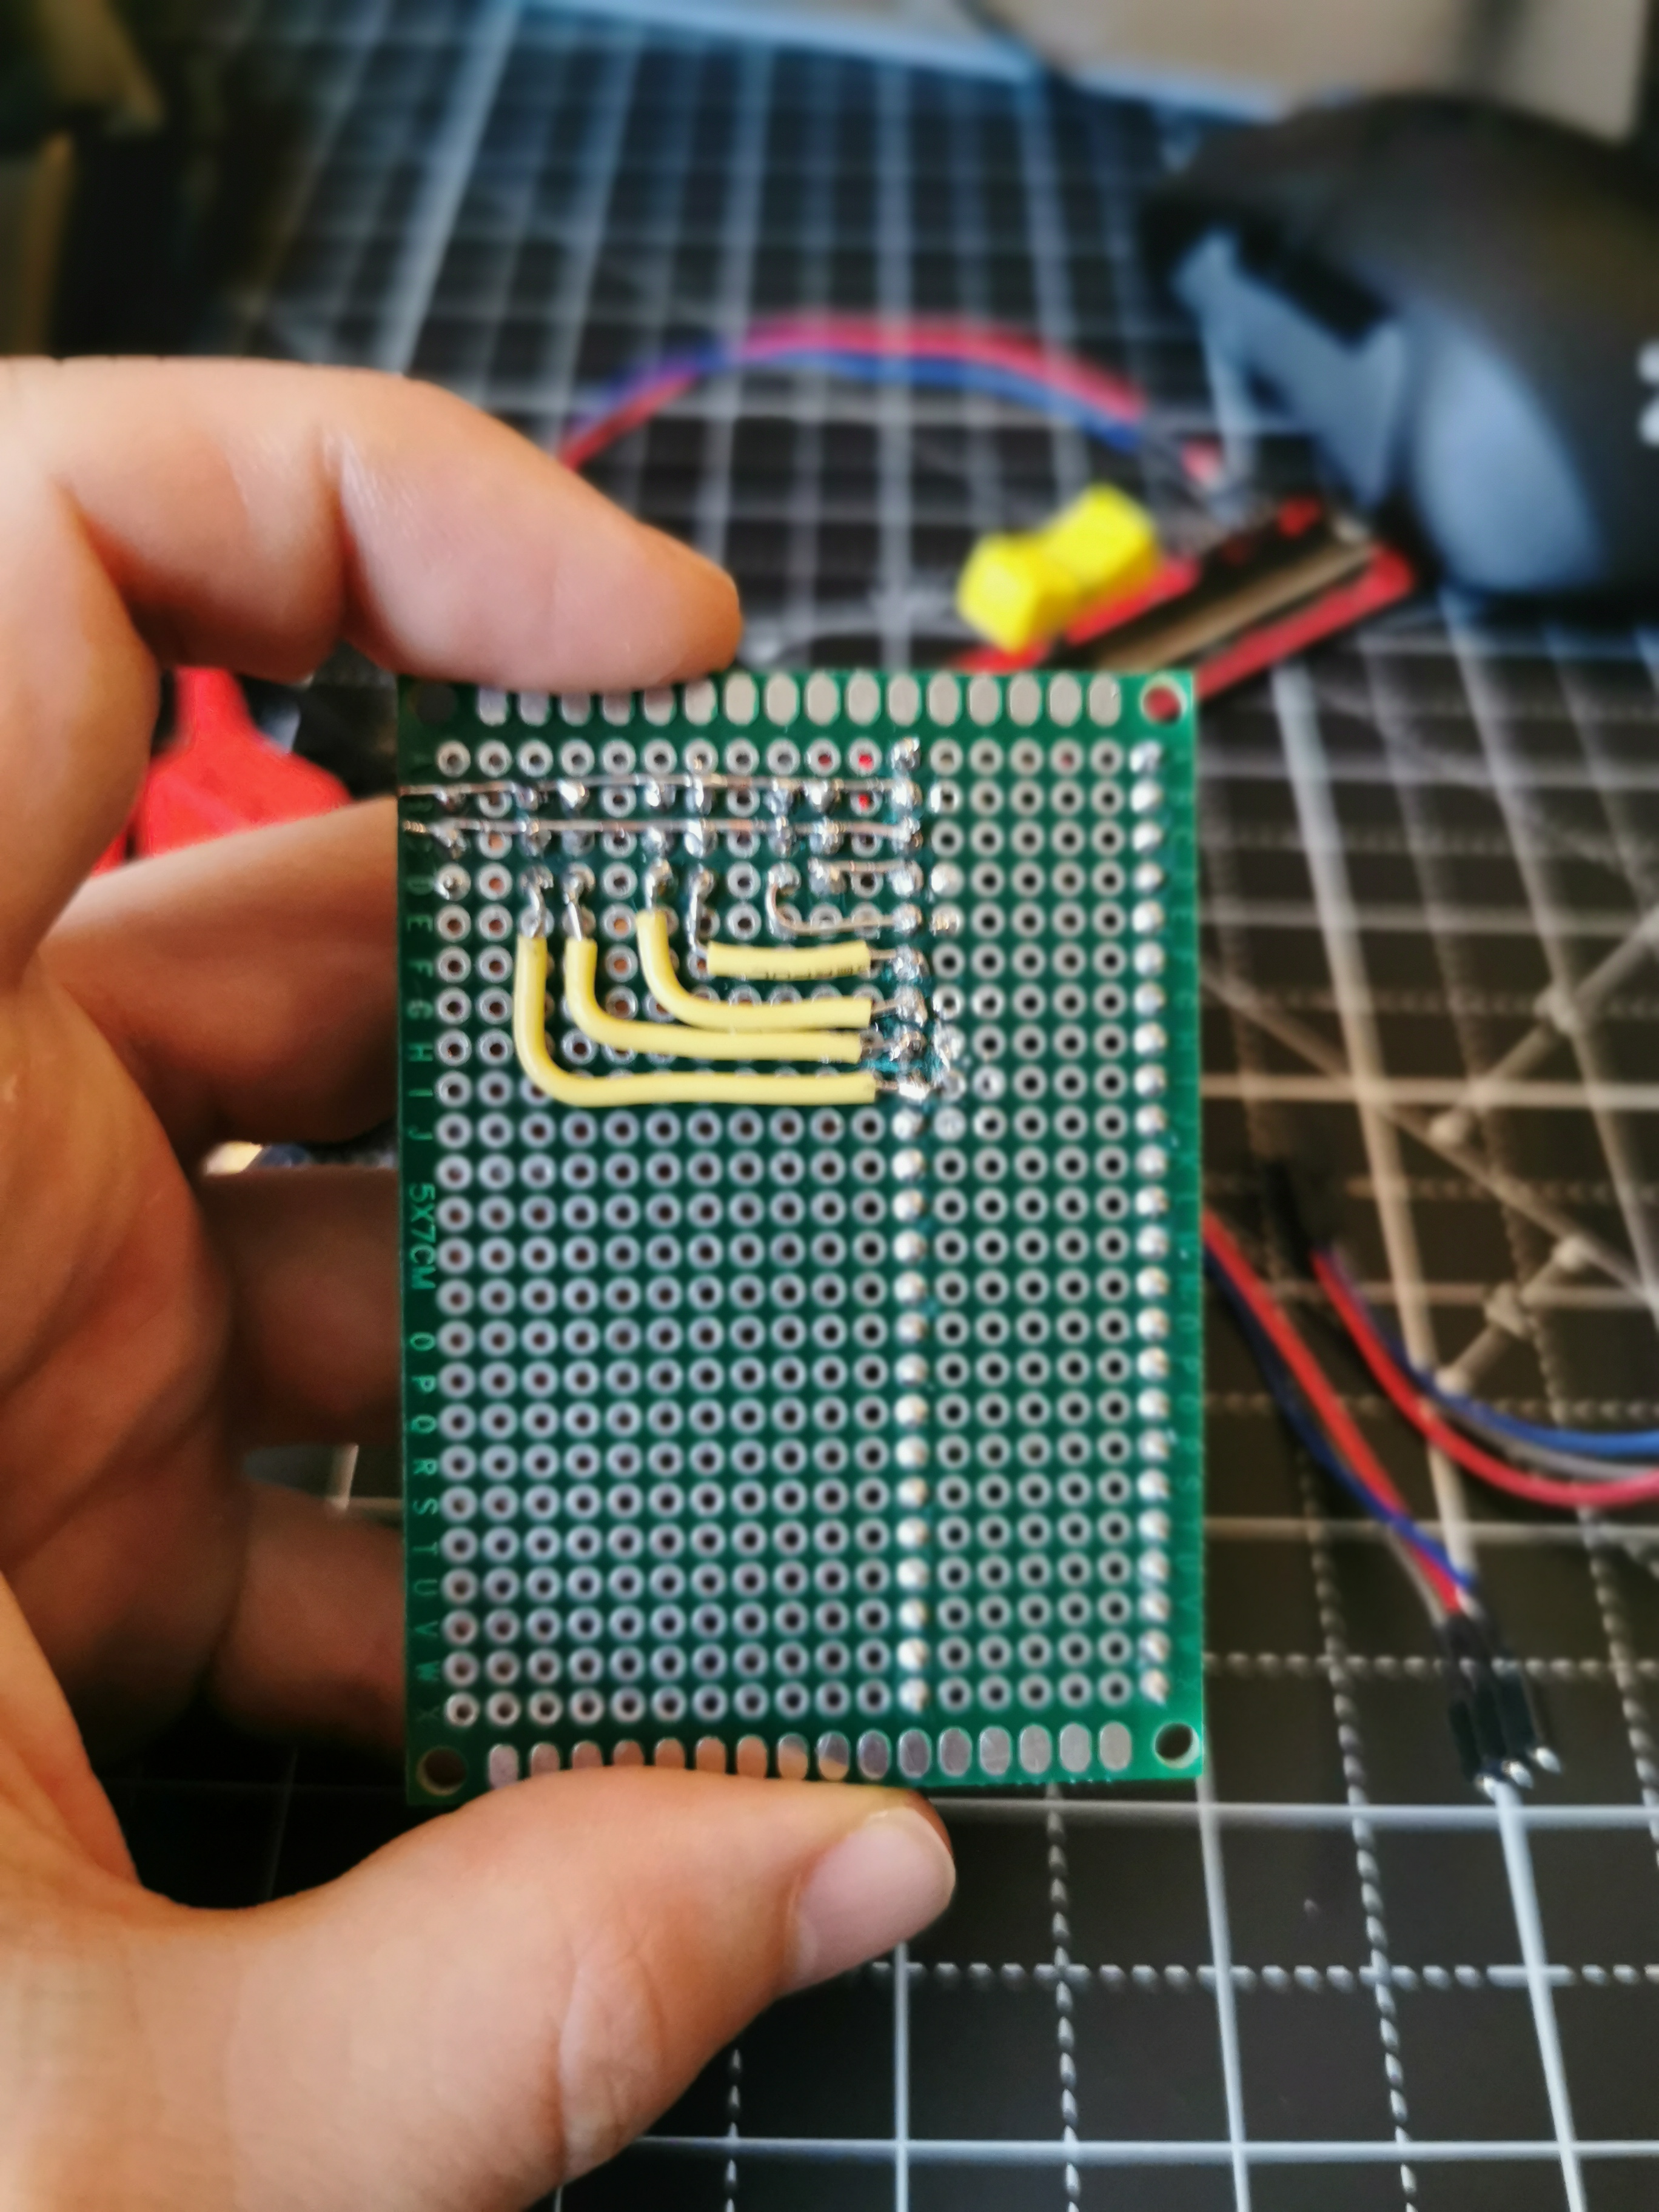
\includegraphics[width=0.74\textwidth]{hw_4}
\captionof{figure}{Lochrasterplatine mit\\Kabelverbindungen}
\end{minipage}
\begin{minipage}[t]{0.5\textwidth}
\centering
\includegraphics[width=0.75\textwidth]{hw_5}
\captionof{figure}{fertgie Verkabelung mit\\Reglern und Teensy}
\end{minipage}\\\\
Um das System modular zu halten, wurden alle Anschlüsse mit Jumperkabeln (Female) realisiert und der Mikrocontroller selbst mit Buchsenleisten auf die Lochrasterplatine gelötet.\\
\begin{figure}[h]
\centering
  \includegraphics[width=0.5\textwidth]{hw_6}
  \caption{Rückseite der Gehäuseblende mit Reglern}
\end{figure}

\newpage

\subsubsection{Gehäuse}

\noindent Nach erfolgreicher Verkabelung wurde ein passendes Gehäuse gestaltet. Dabei wurden eine Holzkonstruktion und der 3D-Druck in Betracht gezogen, wobei die Entscheidung aufgrund der Praktikabilität auf letzteren fiel. Die erste Skizze orientierte sich an der Vision des Projekts. Hinsichtlich des Erscheinungsbildes ähnelten sie den KI generierten.\\
Um den gewünschten Synthesizer-Look zu realisieren, wurden die sechs Drehregler nebenläufig auf dem oberen Teil des Gehäuses angeordnet, gefolgt vom Schieberegler und dem Button darunter. Das erste Gehäuse hatte dann eine Länge, Breite und Höhe von (19 x 9 x 5) cm.\\\\
\begin{minipage}[t]{0.5\textwidth}
\centering
\includegraphics[width=0.85\textwidth]{hw_1}
\captionof{figure}{erste Skizze des Gehäuses}
\end{minipage}
\begin{minipage}[t]{0.5\textwidth}
\centering
\includegraphics[width=0.8\textwidth]{hw_0}
\captionof{figure}{KI generierte Vision aus dem Konzept}
\end{minipage}\\
\\\\
Für die Modellierung kam die Software Fusion360 von AutoDesk zum Einsatz, während die druckereigene Software CraftWare Pro zur Generierung des G-Codes verwendet wurde.\\
\begin{figure}[h]
\centering
  \includegraphics[scale=0.25]{hw_2}
  \caption{3D Modell des Gehäuses in Fusion360}
\end{figure}
\newpage
\noindent Der Teensy fand seinen Platz in einer Fassung im Gehäuse, etwa dort, wo sich der Button befindet. Die Hälse der Drehregler ließen sich durch die Blende schieben und dann auf der gegenüberliegenden Seite mit einer Mutter fixieren. Ebenso wurde der Schieberegler befestigt. Die Verbindung der Blende mit dem unteren Teil des Gehäuses gestaltete sich als aufwendiger. Hier wurden zwei Gewindeeinsätze erhitzt und in das Gehäuse aus PLA-Filament geschmolzen und verschraubt.\\
\begin{figure}[h]
\centering
  \includegraphics[scale=0.5]{hw_3}
  \caption{Finalisierter Controller für den Synthesizer}
\end{figure}

\newpage

\subsection{Touch Designer}

In Touch-Designer war das Ziel interessante, audioreaktive Visuals erzeugen, die den granularen Synthesizer visuell untermalen. Man hatte außerdem den Anspruch, dass zwischen den Visuals automatisch oder manuell umgeschaltet werden kann.

\subsubsection{Gesamtstruktur}

In der Gesamtstruktur des Touch-Designer Files sind die einzelnen Visuals als .tox-Dateien eingefügt. Auf diese Weise können alle Visuals parallel laufen. Am Anfang gibt es einen Audioinput, auf den alle Visuals zugreifen. So wird nicht für jedes Visual ein eigener Input benötigt, sondern alle haben nur einen „In“ Chop, über den sie auf den gleichen Audioinput zugreifen können. Am Ende jeder .tox-Datei ist ein „Out“ Chop, worüber die Ausgänge der Visuals alle in einen „Switch“ laufen. Dieser Switch geht in ein „Cross“.
\begin{wrapfigure}{r}{0.7\textwidth}
  \centering
  \includegraphics[width=0.7\textwidth]{td_1}
  \caption{Struktur des Touch Designer Programms}
\end{wrapfigure}

\noindent In den anderen Eingang des „Cross“ geht ein schwarzes Bild, welches für den Übergang zwischen den Visuals benötigt wird. Am Ausgang des „Cross“ hängt ein „Window“, welches der finale Ausgang für Touch-Designer ist. Für den Übergang gibt es einen automatischen und einen manuellen Modus.
\\\\
Im Automatischen Modus zählt ein Timer hoch, der nach einer bestimmten Zeit den Übergang auslöst. Beim Übergang wechselt der „Cross“ für einen kurzen Moment auf das schwarze Bild. Hier gibt es einen Fade und keinen harten Cut. In dem Moment, indem das Bild Vollständig schwarz wird, springt der „Switch“ auf das nächste Visual und der „Cross“ fadet aus dem schwarzen Bild zurück auf das neue Visual. Für den manuellen Modus gibt es einen extra Knopf auf dem Controller, der ein Midi Signal an Touch-Designer schickt und den Übergang einleitet. Nach dem manuellen Wechsel bleibt das ausgewählte Visual für eine bestimmte Zeit stehen. Läuft diese Zeit ab, ohne dass der Knopf erneut gedrückt wurde, springt Touch-Designer wieder in den automatischen Modus, damit nicht dauerhaft ein Visual stehen bleibt, sobald der Knopf einmal gedrückt wurde. 


\newpage

\subsubsection{Visuals}

\textbf{Color Blobs}\\\\
\begin{minipage}{0.4\textwidth}
In diesem Audio-Visualizer wird das Spektrum des Audio-Inputs genutzt, um Kreise zu erstellen und deren Größe zu verändern. Diese werden durch eine Aneinanderreihung von Feedback, Blur, Displace, Mirror und anderen TOP-Nodes zu einem Interessanten, sich bewegenden „rohrschachtest-artigen“ Muster. Die Farbgebung wird über eine Ramp- und einen Lookup-TOP gesteuert.
\vspace{60pt}
\end{minipage}
\hspace{20pt}
\begin{minipage}{0.5\textwidth}
  \centering
  \includegraphics[width=\textwidth]{td_2}
  \captionof{figure}{„Color Blobs''}
\end{minipage}
\\\\
\textbf{Point Cloud}\\\\
\begin{minipage}{0.4\textwidth}
 Eine Röhre wird verformt und durch ein Noise-TOP geschickt. Das Abbild der Röhre wird dann durch 	eine Point Cloud aus kleinen Quadraten abgebildet. Das Noise wird durch den Audio-Input verändert, 	wodurch die Audio-Reaktivität erzeugt wird.
\vspace{110pt}
\end{minipage}
\hspace{20pt}
\begin{minipage}{0.5\textwidth}
  \centering
  \includegraphics[width=\textwidth]{td_3}
  \captionof{figure}{ „Point Cloud“}
\end{minipage}
\\\\
\\\\
\\\\
\\\\
\textbf{Fuzzy Ball}\\\\
\begin{minipage}{0.4\textwidth}
Hier wird eine verformte Kugel mit einem PHONG-Material versehen, dessen Farbe, Height-Map und Normal-Map, durch ein sich bewegendes Noise erstellt werden. Das Material wird in einer Gitter-Optik angezeigt. Farbe wird in Form von Beleuchtung hinzugefügt. Die Verformung und die Beleuchtungsintensität werden über den Audio-Input gesteuert.
\vspace{90pt}
\end{minipage}
\hspace{20pt}
\begin{minipage}{0.5\textwidth}
  \centering
  \includegraphics[width=\textwidth]{td_4}
  \captionof{figure}{„Fuzzy Ball“}
\end{minipage}
\\\\
\textbf{Purple Fog}\\\\
\begin{minipage}{0.4\textwidth}
Dieses Visual basiert auf einem Circle, dessen Größe auf das Audiosignal reagiert. Zudem wird er durch verschiedene Filter, wie zum Beispiel „Displace“ und „Edge“ in seiner Form verändert. Das Top „Ramp“ sorgt hier für den Farbverlauf. Durch ein „Noise“ wird der Circle noch stärker verzerrt und es entsteht dann die Finale Struktur. Um den Effekt zu verstärken, wird anschließend ein Feedback Loop eingebaut.
\vspace{1pt}
\end{minipage}
\hspace{20pt}
\begin{minipage}{0.5\textwidth}
  \centering
  \includegraphics[width=\textwidth]{td_6}
  \captionof{figure}{„Purple Fog“}
\end{minipage}
\newpage
\noindent\textbf{Donut}
\begin{wrapfigure}{r}{0.7\textwidth}
  \centering
  \includegraphics[width=0.6\textwidth]{td_5}
  \caption{„Donut“}
\end{wrapfigure}

\noindent Für den Hintergrund wird ein Circle genutzt, aus dem mittels eines „Noise“ Tops eine Wolke aus vielen Kugeln erstellt wird. In diese Wolke wird die Kamera platziert, um den Effekt einer Galaxie zu erzeugen. Für die Wolke wird nun ein Loop erstellt, sodass sich die Kugeln auf die Kamera zu bewegen. Sobald eine bestimmte Position hinter der Kamera erreicht ist, springen die Kugeln wieder auf die Startposition zurück und es entsteht ein Effekt, in dem Kugeln permanent auf die Kamera zu fliegen. Die Geschwindigkeit der Kugeln wird durch den Audioinput beeinflusst. In dieses Feld wird ein Torus eingefügt, welcher durch das „Line Material“ seine Struktur erhält. Damit der Torus durch das Audiosignal verändert werden kann, reagiert zum einen die Größe des Torus auf das Eingangssignal und zum anderen wird ein „Noise“ dazu geschaltet, dessen Amplitude ebenfalls auf das Eingangssignal reagiert. Durch das „Noise“ kommt es zu den Änderungen in der Struktur des Torus.

\subsection{Zusätzliche Software zum Verbinden von SunVox und Touch Designer}

Damit Touch-Designer das Audio aus Sunvox empfangen kann, muss entweder ein Loopback-fähiges Audiointerface oder eine weitere Software genutzt werden. Man hat sich nach einigem Ausprobieren für die Software VB-Cable entschieden, welche als virtuelles Audiokabel dient, mit dem sich der Output von Sunvox in den Input von Touch-Designer leiten lässt.
\\\\
Ein weiteres Problem war, dass in Windows nur ein Programm zur Zeit von einem MIDI-Controller angesteuert werden kann. Man wollte allerdings Sunvox und Touch-Designer über den gleichen MIDI-Controller ansteuern. Hierfür war eine Kombination aus zwei zusätzlichen Softwares nötig. Die Software loopMidi wird genutzt, um zwei virtuelle MIDI-Geräte für jeweils Sunvox und Touch-Designer zu erzeugen. Dann wird mit der Software MIDI-OX das angeschlossene MIDI-Gerät in die beiden virtuellen MIDI-Geräte geleitet.
So ist es Möglich, dass die Audio-Visualizer in Touch-Designer auf das Audio aus Sunvox reagieren können und mit einem einzelnen MIDI-Controller beide Softwares angesteuert werden können.

\section{Fazit}

\subsection{Zusammenfassung}

\subsubsection{SunVox}

Zu SunVox lässt sich insgesamt sagen, dass es für Audiosynthese und elektronische Musik für ein kostenloses Programm ein mächtiges Werkzeug ist. Leider ist es eher darauf programmiert, Songs zu gestalten und zu produzieren und weniger, selbst als Instrument genutzt zu werden. Das führte dazu, dass in der Ausgestaltung der Installation einige Kompromisse vereinbart werden mussten, da einfache Funktionen wie ein Shortcut zur Aufnahme von Samples in der Software nicht vorhanden sind. Jedoch lässt sich, in Bezug auf den Synthesizer, ein positives Bild ziehen. Trotz der teilweise umständlichen Steuerung von SunVox ist das Ergebnis ein guter Granular Synthesizer, der sich kreativ spielen lässt und mit den Visuals aus TouchDesigner harmoniert.

\subsubsection{Touch Designer}

Nach ein paar Wochen, die man im Touch Designer Gewerk brauchte, um sich in der Software zurecht zu finden, hat man angefangen selbst Visuals zu bauen. Von diesen wurden sechs ausgesucht, zwischen denen im Finalen Projekt umgeschaltet werden konnte. Zusätzlich hätte man gern in Touch-Designer noch mehr MIDI-Daten des Controllers eingebunden und Lichter im Raum über DMX angesteuert. Die wichtigsten Funktionalitäten, konnten aber gut umsetzt werden. 

\subsection{Ausblick}

Trotz der Tatsache, dass man mit dem Ergebnis zufrieden sein kann, gibt es einige Punkte, die noch umgesetzt werden können bzw. die einem für Austellungen geeignetem VisuSynth (z.B. auf dem Rundgang Finkenau) beitragen würden:
\begin{itemize}
  \item Die Aufnahme über den Mikrocontroller ansteuern mit dem Ziel das Setup ohne Laptopdisplay, Maus und Tastatur umzusetzen.
  \item Ein kleines Display auf dem die Waveform der Aufnahme angezeigt wird.
  \item Eine Möglichkeit zum Spielen von Noten in den MIDI-Controller einbauen . So wäre das zusätzliche MIDI-Keyboard nicht nötig.
   \item Einen Reset-Knopf einbauen, falls ein unerträglicher Sound erzeugt wurde oder gar nichts passiert.
   \item Einbindung der MIDI-Parameter in die Touch-Designer-Visuals.
   \item Licht für die Installation über DMX audioreaktiv ansteuern.
   \item Mehr Visuals und reaktivere Visuals (häufig haben sie nur bei viel Bass stark reagiert).

\end{itemize}

\section{Quellenverzeichnis}

\textbf{Grundlagen}
\\\\
Native Instruments (2023): Granular synthesis: a beginner’s guide.\\
URL: \href{https://blog.native-instruments.com/granular-synthesis/}{https://blog.native-instruments.com/granular-synthesis/}
\\\\
Opie, Tallaine (1999-2023): Granular Synthesis Resource Site.\\
URL: \href{http://www.granularsynthesis.com/guide.php}{http://www.granularsynthesis.com/guide.php}
\\\\
Nicole (2022): A Brief History Of Synthesizers.\\
URL: \href{https://www.hi5electronics.co.uk/a-brief-history-of-synthesizers/}{https://www.hi5electronics.co.uk/a-brief-history-of-synthesizers/}
\\\\
Meierhans, Hermann Josef (2022): Wie liest man MIDI-Codes? Einfach erklärt!\\
URL: \href{https://www.amazona.de/workshop-das-midi-datenformat-einfach-erklaert/}{https://www.amazona.de/workshop-das-midi-datenformat-einfach-erklaert/}
\\\\
\textbf{SunVox}
\\\\
Zolotov, Alexander (2023): SunVox User Manual.\\
URL: \href{https://warmplace.ru/soft/sunvox/manual.php}{https://warmplace.ru/soft/sunvox/manual.php}
\\\\
\textbf{Touch Designer}
\\\\
Olea, Pao (2023): Fluffy material.\\
URL: \href{https://www.youtube.com/watch?v=rcrW-A27VYo}{https://www.youtube.com/watch?v=rcrW-A27VYo}
\\\\
Acrylicode (2023): Audio-reactive psychedelic visuals.\\
URL: \href{https://www.youtube.com/watch?v=Mt2hwb5cngA}{https://www.youtube.com/watch?v=Mt2hwb5cngA}
\\\\
Smih, Jeffrey (2011): transition between projects in performance.\\
URL: \href{https://forum.derivative.ca/t/transition-between-projects-in-performance/2573}{https://forum.derivative.ca/t/transition-between-projects-in-performance/2573}
\\\\
Derivative Inc. (2019): TouchDesigner User Guide.\\
URL: \href{https://docs.derivative.ca/}{https://docs.derivative.ca/}
\\\\
Acrylicode (2023): Audio reactive Galaxy.\\
URL: \href{https://www.youtube.com/watch?v=J7s7aK2M3mw}{https://www.youtube.com/watch?v=J7s7aK2M3mw}
\\\\
Steenhoff, Daniel (2023): Audioreactive Fluid Grid VISUAL.\\
URL: \href{https://www.youtube.com/watch?v=Hu_81_WOlCo}{$\mathrm{https://www.youtube.com/watch?v=Hu_81_WOlCo}$}
\\\\
\textbf{Zusätzliche Software}
\\\\
O'Connell, Jamie (1997-2018): MIDI-OX.\\
URL: \href{http://www.midiox.com/}{http://www.midiox.com/}
\\\\
Erichsen, Tobias (2010-2022): loopMIDI.\\
URL: \href{https://www.tobias-erichsen.de/software/loopmidi.html}{https://www.tobias-erichsen.de/software/loopmidi.html}
\\\\
Burel, Vincent (1999-2023): VB-Cable.\\
URL: \href{https://vb-audio.com/Cable/}{https://vb-audio.com/Cable/}


\end{document}